% Options for packages loaded elsewhere
\PassOptionsToPackage{unicode}{hyperref}
\PassOptionsToPackage{hyphens}{url}
%
\documentclass[
]{book}
\usepackage{amsmath,amssymb}
\usepackage{lmodern}
\usepackage{ifxetex,ifluatex}
\ifnum 0\ifxetex 1\fi\ifluatex 1\fi=0 % if pdftex
  \usepackage[T1]{fontenc}
  \usepackage[utf8]{inputenc}
  \usepackage{textcomp} % provide euro and other symbols
\else % if luatex or xetex
  \usepackage{unicode-math}
  \defaultfontfeatures{Scale=MatchLowercase}
  \defaultfontfeatures[\rmfamily]{Ligatures=TeX,Scale=1}
\fi
% Use upquote if available, for straight quotes in verbatim environments
\IfFileExists{upquote.sty}{\usepackage{upquote}}{}
\IfFileExists{microtype.sty}{% use microtype if available
  \usepackage[]{microtype}
  \UseMicrotypeSet[protrusion]{basicmath} % disable protrusion for tt fonts
}{}
\makeatletter
\@ifundefined{KOMAClassName}{% if non-KOMA class
  \IfFileExists{parskip.sty}{%
    \usepackage{parskip}
  }{% else
    \setlength{\parindent}{0pt}
    \setlength{\parskip}{6pt plus 2pt minus 1pt}}
}{% if KOMA class
  \KOMAoptions{parskip=half}}
\makeatother
\usepackage{xcolor}
\IfFileExists{xurl.sty}{\usepackage{xurl}}{} % add URL line breaks if available
\IfFileExists{bookmark.sty}{\usepackage{bookmark}}{\usepackage{hyperref}}
\hypersetup{
  pdftitle={Ten SPSS tricks to make your peers jealous},
  pdfauthor={Bernard Liew},
  hidelinks,
  pdfcreator={LaTeX via pandoc}}
\urlstyle{same} % disable monospaced font for URLs
\usepackage{color}
\usepackage{fancyvrb}
\newcommand{\VerbBar}{|}
\newcommand{\VERB}{\Verb[commandchars=\\\{\}]}
\DefineVerbatimEnvironment{Highlighting}{Verbatim}{commandchars=\\\{\}}
% Add ',fontsize=\small' for more characters per line
\usepackage{framed}
\definecolor{shadecolor}{RGB}{248,248,248}
\newenvironment{Shaded}{\begin{snugshade}}{\end{snugshade}}
\newcommand{\AlertTok}[1]{\textcolor[rgb]{0.94,0.16,0.16}{#1}}
\newcommand{\AnnotationTok}[1]{\textcolor[rgb]{0.56,0.35,0.01}{\textbf{\textit{#1}}}}
\newcommand{\AttributeTok}[1]{\textcolor[rgb]{0.77,0.63,0.00}{#1}}
\newcommand{\BaseNTok}[1]{\textcolor[rgb]{0.00,0.00,0.81}{#1}}
\newcommand{\BuiltInTok}[1]{#1}
\newcommand{\CharTok}[1]{\textcolor[rgb]{0.31,0.60,0.02}{#1}}
\newcommand{\CommentTok}[1]{\textcolor[rgb]{0.56,0.35,0.01}{\textit{#1}}}
\newcommand{\CommentVarTok}[1]{\textcolor[rgb]{0.56,0.35,0.01}{\textbf{\textit{#1}}}}
\newcommand{\ConstantTok}[1]{\textcolor[rgb]{0.00,0.00,0.00}{#1}}
\newcommand{\ControlFlowTok}[1]{\textcolor[rgb]{0.13,0.29,0.53}{\textbf{#1}}}
\newcommand{\DataTypeTok}[1]{\textcolor[rgb]{0.13,0.29,0.53}{#1}}
\newcommand{\DecValTok}[1]{\textcolor[rgb]{0.00,0.00,0.81}{#1}}
\newcommand{\DocumentationTok}[1]{\textcolor[rgb]{0.56,0.35,0.01}{\textbf{\textit{#1}}}}
\newcommand{\ErrorTok}[1]{\textcolor[rgb]{0.64,0.00,0.00}{\textbf{#1}}}
\newcommand{\ExtensionTok}[1]{#1}
\newcommand{\FloatTok}[1]{\textcolor[rgb]{0.00,0.00,0.81}{#1}}
\newcommand{\FunctionTok}[1]{\textcolor[rgb]{0.00,0.00,0.00}{#1}}
\newcommand{\ImportTok}[1]{#1}
\newcommand{\InformationTok}[1]{\textcolor[rgb]{0.56,0.35,0.01}{\textbf{\textit{#1}}}}
\newcommand{\KeywordTok}[1]{\textcolor[rgb]{0.13,0.29,0.53}{\textbf{#1}}}
\newcommand{\NormalTok}[1]{#1}
\newcommand{\OperatorTok}[1]{\textcolor[rgb]{0.81,0.36,0.00}{\textbf{#1}}}
\newcommand{\OtherTok}[1]{\textcolor[rgb]{0.56,0.35,0.01}{#1}}
\newcommand{\PreprocessorTok}[1]{\textcolor[rgb]{0.56,0.35,0.01}{\textit{#1}}}
\newcommand{\RegionMarkerTok}[1]{#1}
\newcommand{\SpecialCharTok}[1]{\textcolor[rgb]{0.00,0.00,0.00}{#1}}
\newcommand{\SpecialStringTok}[1]{\textcolor[rgb]{0.31,0.60,0.02}{#1}}
\newcommand{\StringTok}[1]{\textcolor[rgb]{0.31,0.60,0.02}{#1}}
\newcommand{\VariableTok}[1]{\textcolor[rgb]{0.00,0.00,0.00}{#1}}
\newcommand{\VerbatimStringTok}[1]{\textcolor[rgb]{0.31,0.60,0.02}{#1}}
\newcommand{\WarningTok}[1]{\textcolor[rgb]{0.56,0.35,0.01}{\textbf{\textit{#1}}}}
\usepackage{longtable,booktabs,array}
\usepackage{calc} % for calculating minipage widths
% Correct order of tables after \paragraph or \subparagraph
\usepackage{etoolbox}
\makeatletter
\patchcmd\longtable{\par}{\if@noskipsec\mbox{}\fi\par}{}{}
\makeatother
% Allow footnotes in longtable head/foot
\IfFileExists{footnotehyper.sty}{\usepackage{footnotehyper}}{\usepackage{footnote}}
\makesavenoteenv{longtable}
\usepackage{graphicx}
\makeatletter
\def\maxwidth{\ifdim\Gin@nat@width>\linewidth\linewidth\else\Gin@nat@width\fi}
\def\maxheight{\ifdim\Gin@nat@height>\textheight\textheight\else\Gin@nat@height\fi}
\makeatother
% Scale images if necessary, so that they will not overflow the page
% margins by default, and it is still possible to overwrite the defaults
% using explicit options in \includegraphics[width, height, ...]{}
\setkeys{Gin}{width=\maxwidth,height=\maxheight,keepaspectratio}
% Set default figure placement to htbp
\makeatletter
\def\fps@figure{htbp}
\makeatother
\setlength{\emergencystretch}{3em} % prevent overfull lines
\providecommand{\tightlist}{%
  \setlength{\itemsep}{0pt}\setlength{\parskip}{0pt}}
\setcounter{secnumdepth}{5}
\usepackage{booktabs}
\ifluatex
  \usepackage{selnolig}  % disable illegal ligatures
\fi
\usepackage[]{natbib}
\bibliographystyle{apalike}

\title{Ten SPSS tricks to make your peers jealous}
\author{Bernard Liew}
\date{2021-05-12}

\begin{document}
\maketitle

{
\setcounter{tocdepth}{1}
\tableofcontents
}
\hypertarget{introduction}{%
\chapter*{Introduction}\label{introduction}}
\addcontentsline{toc}{chapter}{Introduction}

Most people interact with SPSS using what I call the ``point and click'' interface. A point-click method is not wrong per-se, I use it. The bad thing about the point-click method is that:

\begin{enumerate}
\def\labelenumi{\arabic{enumi})}
\item
  You cannot easily remember what you did. Try recalling the exact order of actions you undertook the last time you analyzed your data in SPSS. It is for this reason why one gets nervous reproducing the results.
\item
  It gets tedious really quickly, especially if you want to do the same thing repeatedly.
\end{enumerate}

The alternative to the ``point and click'' interface, is using the \textbf{SPSS syntax}. Syntax is all about typing. You can open a fresh syntax like in \ref{fig:first-syntax}, populate it with commands to run, and save it. My rule of thumb is, when you spend so long getting something commands running, save your commands, not your results.

\begin{figure}
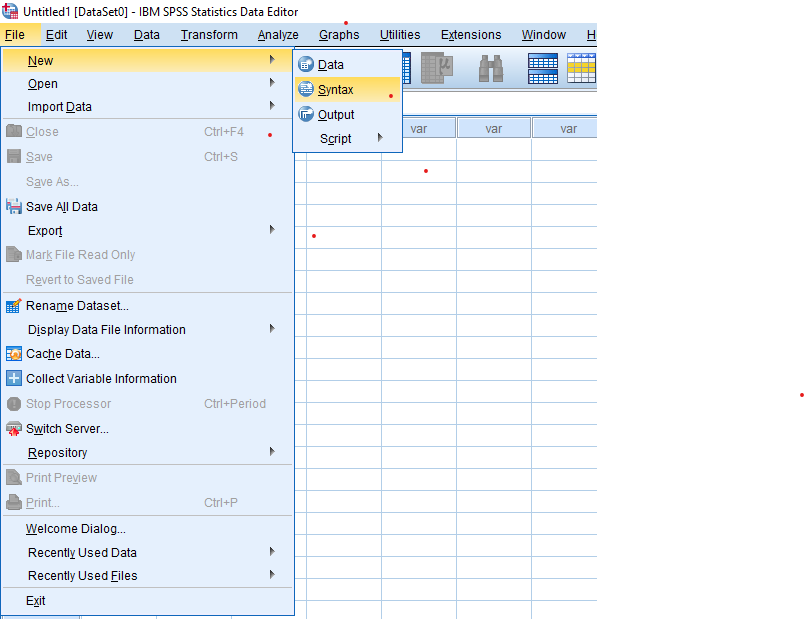
\includegraphics[width=0.5\linewidth]{images/open_syntax} \caption{Open your first syntax}\label{fig:first-syntax}
\end{figure}

\hypertarget{trick-1---paste-to-syntax}{%
\chapter*{Trick 1 - Paste to syntax}\label{trick-1---paste-to-syntax}}
\addcontentsline{toc}{chapter}{Trick 1 - Paste to syntax}

The good thing about interacting with SPSS using syntax, is that you do not have to be a total convert. You can continue using the ``point and click'' interface, but instead of executing the command, press \textbf{paste} as you see in Figure \ref{fig:paste-syntax}. Pasting automatically copies the word version of what you clicked into your opened syntax.

\begin{figure}
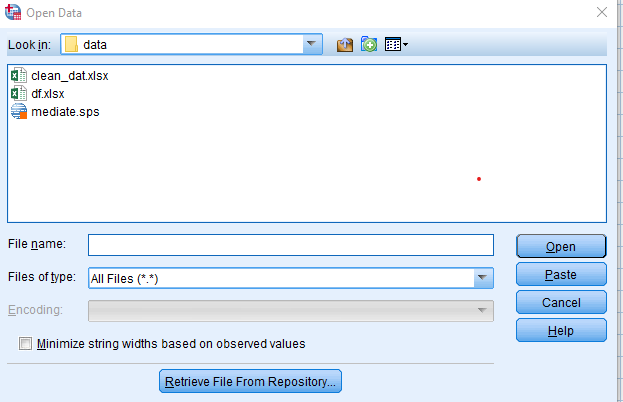
\includegraphics[width=0.6\linewidth]{images/paste_syntax} \caption{Paste the syntax you generated implicitly by clicking}\label{fig:paste-syntax}
\end{figure}

I have not ever encountered an SPSS function that does not eventually have a paste function. Try finding it and saving what you intend to do like in Figure \ref{fig:paste-syntax2}.

\begin{figure}
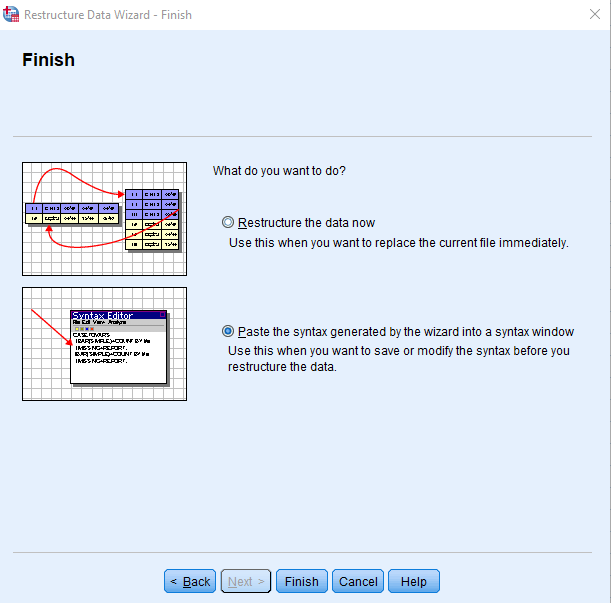
\includegraphics[width=0.5\linewidth]{images/paste_syntax2} \caption{Always try to paste your syntax rather than executing}\label{fig:paste-syntax2}
\end{figure}

To run each command, highlight and press the play button like in Figure \ref{fig:play}.

\begin{figure}
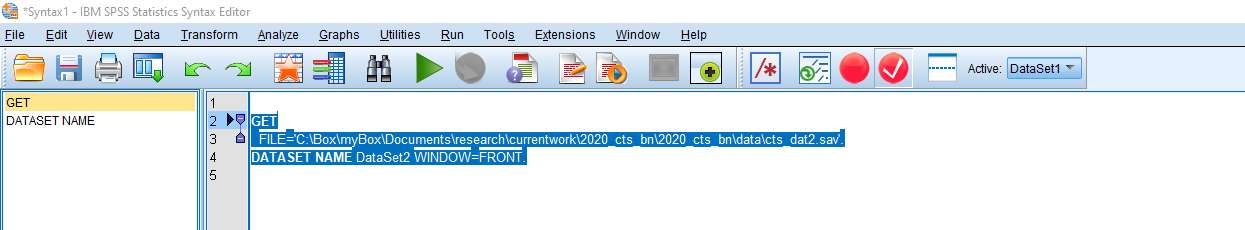
\includegraphics[width=0.8\linewidth]{images/run_syntax} \caption{Executing a command}\label{fig:play}
\end{figure}

\hypertarget{trick-2---setting-your-work-directory}{%
\chapter*{Trick 2 - Setting your work directory}\label{trick-2---setting-your-work-directory}}
\addcontentsline{toc}{chapter}{Trick 2 - Setting your work directory}

When importing data from deeply nested folders, it can be a pain to do so. In addition, when exporting files or figures, many often scratch their head as to where the files went to. The solution to this is to \textbf{explicitly} define the folder on your computer where every thing starts and ends. All the files will be exported to that folder. And importing becomes a breeze.

You can set the working directory by pasting the command below into your SPSS syntax, and change the folder path to your path. Just make sure to enclose it in \texttt{"\ "}.

Highlight this command and press the play button.

\begin{Shaded}
\begin{Highlighting}[]
\NormalTok{cd }\StringTok{\textquotesingle{}C:\textbackslash{}Box\textbackslash{}myBox\textbackslash{}Documents}\SpecialCharTok{\textbackslash{}t}\StringTok{eaching\textbackslash{}SE738\textbackslash{}spss\textquotesingle{}}\NormalTok{.}
\end{Highlighting}
\end{Shaded}

\hypertarget{trick-3---importing-data}{%
\chapter*{Trick 3 - Importing data}\label{trick-3---importing-data}}
\addcontentsline{toc}{chapter}{Trick 3 - Importing data}

The most common starting point for data analysis is Excel, so I will demonstrate how to easily import an Excel file. Paste the command below into your syntax, and simply change the file name \texttt{df.xlsx} to whatever your file is named. Remember not to change the file extension \texttt{.xlsx}. If your Excel file has multiple sheets, change the sheet name \texttt{jump} to whatever it is named. If you only have one sheet, you can leave it blank.

Highlight this command and press the play button.

\begin{Shaded}
\begin{Highlighting}[]
\NormalTok{GET DATA}
  \SpecialCharTok{/}\NormalTok{TYPE}\OtherTok{=}\NormalTok{XLSX}
  \SpecialCharTok{/}\NormalTok{FILE}\OtherTok{=} \StringTok{\textquotesingle{}df.xlsx\textquotesingle{}}
  \SpecialCharTok{/}\NormalTok{SHEET}\OtherTok{=}\NormalTok{name }\StringTok{\textquotesingle{}jump\textquotesingle{}}
  \SpecialCharTok{/}\NormalTok{CELLRANGE}\OtherTok{=}\NormalTok{FULL}
  \SpecialCharTok{/}\NormalTok{READNAMES}\OtherTok{=}\NormalTok{ON}
  \SpecialCharTok{/}\NormalTok{DATATYPEMIN PERCENTAGE}\OtherTok{=}\FloatTok{95.0}
  \SpecialCharTok{/}\NormalTok{HIDDEN IGNORE}\OtherTok{=}\NormalTok{YES.}
\end{Highlighting}
\end{Shaded}

Using the sample data I provide, this is what the data looks like in Figure \ref{fig:original}.

\begin{figure}
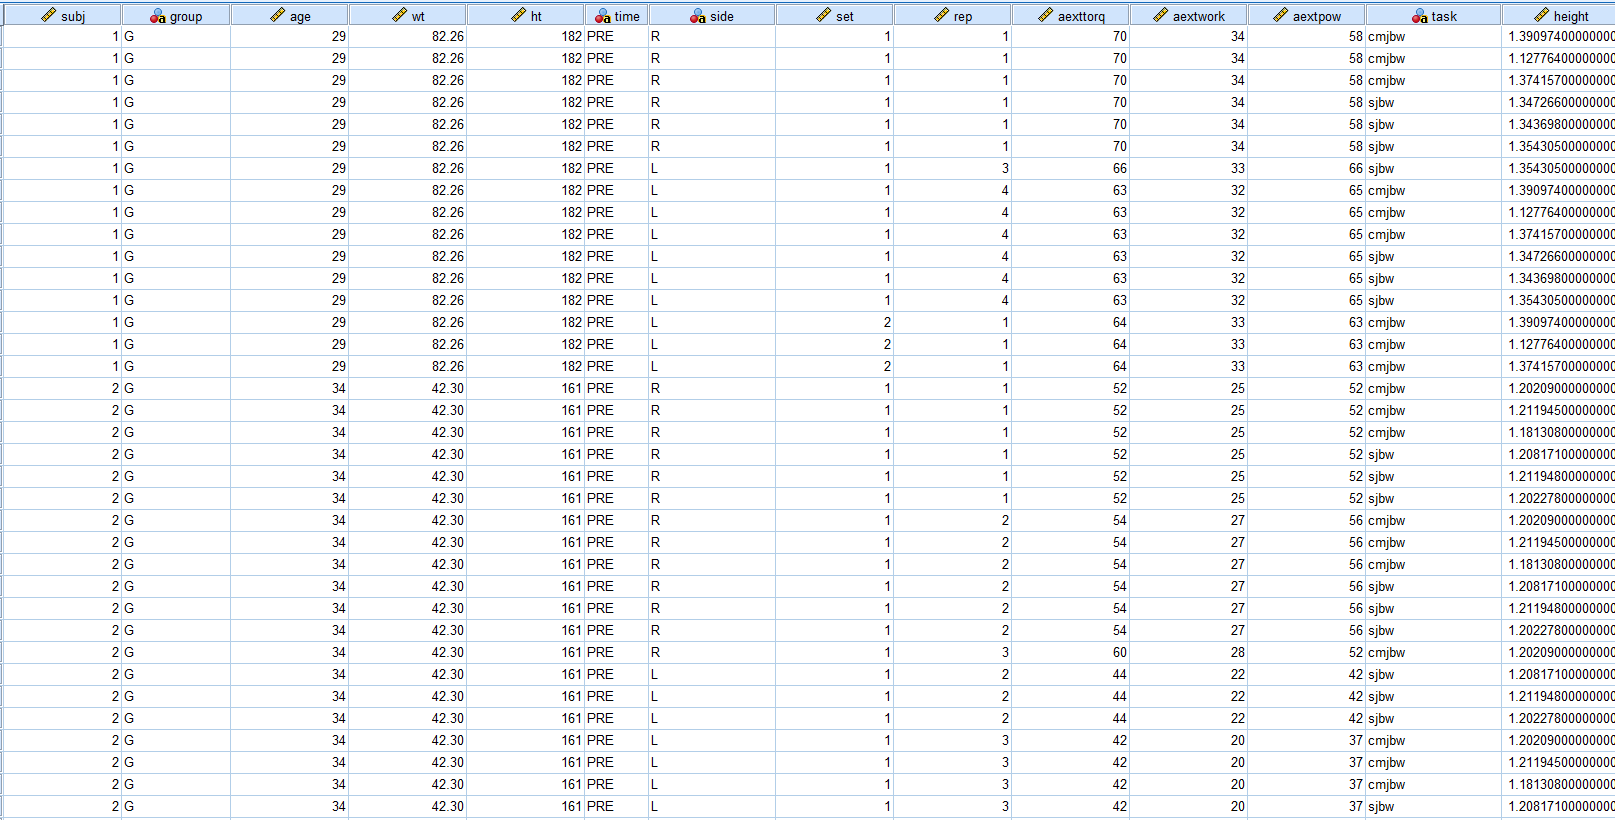
\includegraphics[width=1\linewidth]{images/original_data} \caption{Original data}\label{fig:original}
\end{figure}

\hypertarget{trick-4---rename-columns}{%
\chapter*{Trick 4 - Rename columns}\label{trick-4---rename-columns}}
\addcontentsline{toc}{chapter}{Trick 4 - Rename columns}

Rename columns is a common task. Paste the command below into your syntax and run it. Put all the original column names before the \texttt{=} and all the new names after. There must be a spacing between each name, and the order preceding and proceding the \texttt{=} must be identical.

\begin{Shaded}
\begin{Highlighting}[]
\NormalTok{RENAME }\FunctionTok{VARIABLES}\NormalTok{ (subj group }\AttributeTok{wt  =}\NormalTok{ id grp weight).}
\end{Highlighting}
\end{Shaded}

After renaming this is what the data looks like in Figure \ref{fig:rename-col}.

\begin{figure}
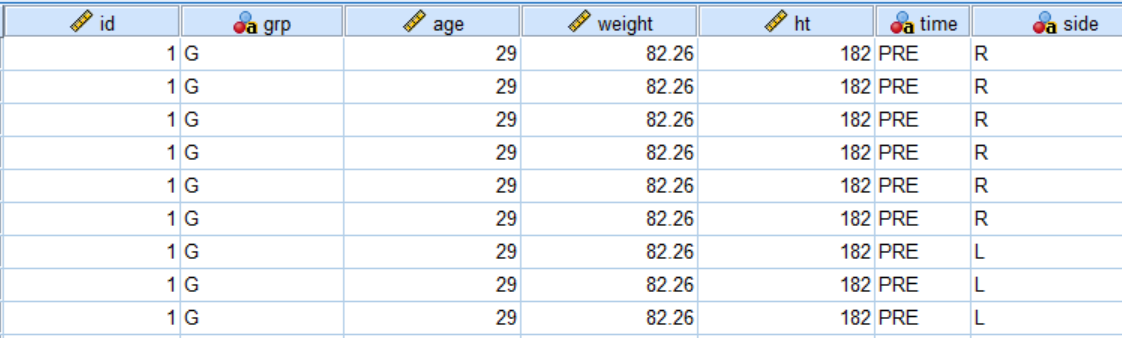
\includegraphics[width=1\linewidth]{images/rename} \caption{New column names}\label{fig:rename-col}
\end{figure}

\hypertarget{trick-5---filter-rows}{%
\chapter*{Trick 5 - Filter rows}\label{trick-5---filter-rows}}
\addcontentsline{toc}{chapter}{Trick 5 - Filter rows}

You might want to keep rows in your data based on some conditions. I tend to prefer to keep whatever rows I want and discard the remaining. Discarding your data does not harm your original data in Excel. If you change your mind, just highlight all the commands from the start and press the play button. In the example below, I want to keep rows where the variable \texttt{task} is equal \texttt{"cmjbw"} AND \texttt{side} is equal to ``\texttt{R}''. Below are some of the operators you can mix and match to powerfully filter our your data.

\textbf{Symbols}

\texttt{=} Equal

\texttt{\textasciitilde{}=} Not equal

\texttt{\textless{}} Less than

\texttt{\textless{}=} Less than or equal

\texttt{\textgreater{}} More than

\texttt{\textgreater{}=} More than or equal

\texttt{\&} AND

\texttt{\textbar{}} OR

Highlight this command and press the play button.

\begin{Shaded}
\begin{Highlighting}[]
\NormalTok{FILTER OFF.}
\NormalTok{USE ALL.}
\NormalTok{SELECT }\FunctionTok{IF}\NormalTok{ (}\AttributeTok{task =} \StringTok{"cmjbw"} \SpecialCharTok{\&}  \AttributeTok{side =} \StringTok{"R"}\NormalTok{).}
\NormalTok{EXECUTE.}
\end{Highlighting}
\end{Shaded}

After filtering this is what the data looks like in Figure \ref{fig:filter-row}.

\begin{figure}
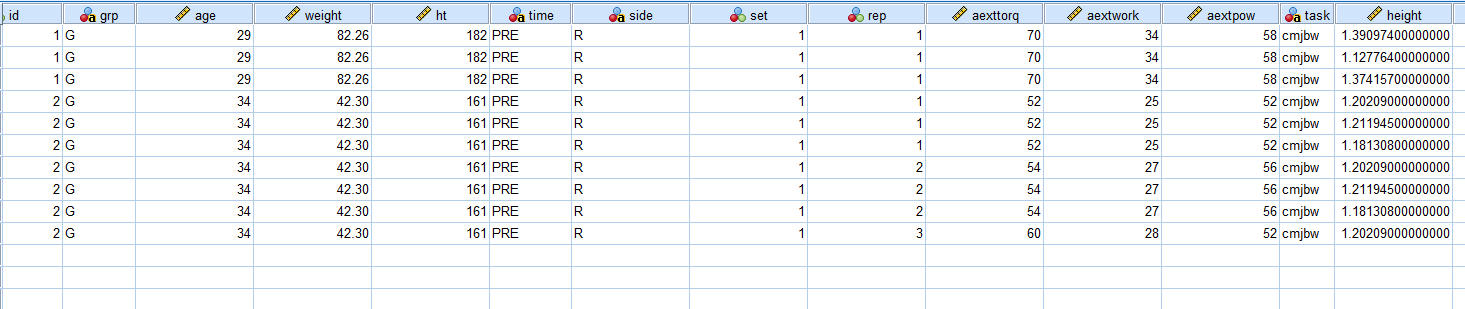
\includegraphics[width=1\linewidth]{images/filter} \caption{Keeping rows based on some conditions}\label{fig:filter-row}
\end{figure}

\hypertarget{trick-6---create-new-variables}{%
\chapter*{Trick 6 - Create new variables}\label{trick-6---create-new-variables}}
\addcontentsline{toc}{chapter}{Trick 6 - Create new variables}

You might want to create new variables, such as calculating BMI from height and mass. Add as many \texttt{COMPUTE} function below as needed. The command reads as \texttt{COMPUTE\ height\ =\ ht/100.}, make a new variable called \texttt{height} by dividing the original variable\texttt{ht} by 100. You can either create a new variable or replace the existing variable by using a new name or the original name, respectively.

\textbf{Math functions}

\texttt{+} Add

\texttt{-} Subtract

\texttt{/} Divide

\texttt{*} Multiply

\texttt{**} Power

Highlight this command and press the play button.

\begin{Shaded}
\begin{Highlighting}[]
\NormalTok{COMPUTE height }\OtherTok{=}\NormalTok{ ht}\SpecialCharTok{/}\FloatTok{100.} 
\NormalTok{COMPUTE weight }\OtherTok{=}\NormalTok{ weight}\SpecialCharTok{/}\FloatTok{100.}
\NormalTok{COMPUTE BMI }\OtherTok{=}\NormalTok{ weight}\SpecialCharTok{/}\NormalTok{(height}\SpecialCharTok{**}\DecValTok{2}\NormalTok{).}
\NormalTok{EXECUTE.}
\end{Highlighting}
\end{Shaded}

After computing new variables this is what the data looks like in Figure \ref{fig:mutate}.

\begin{figure}
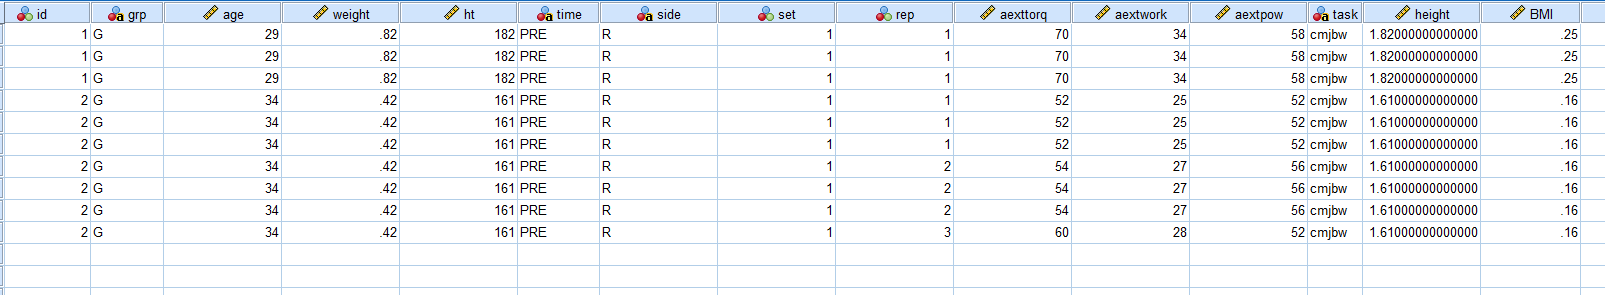
\includegraphics[width=1\linewidth]{images/mutate} \caption{New variables created}\label{fig:mutate}
\end{figure}

\hypertarget{trick-7---aggregate-data}{%
\chapter*{Trick 7 - Aggregate data}\label{trick-7---aggregate-data}}
\addcontentsline{toc}{chapter}{Trick 7 - Aggregate data}

You may want to find some summary statistics for each level of a grouping variable. In the example below, I want to calculate for each id, in each group, at each time, find the mean (\texttt{MEAN}), minimum (\texttt{MIN}), maximum (\texttt{MAX}), standard deviation (\texttt{SD}), and median (\texttt{MEDIAN}) of the following variables (\texttt{aexttorq}, \texttt{aextwork}, \texttt{aextpow}). When you see this argument, \texttt{/aexttorq\_mean=MEAN(aexttorq)}, the value before \texttt{=} represents the new variable name. However many aggregate values you desire, add as many arguments on a separate line. In this command, the aggregate data is pasted onto a separate data window called \texttt{aggregate\_data} - you can give the new data window any name.

\begin{Shaded}
\begin{Highlighting}[]
\NormalTok{DATASET DECLARE aggregate\_data.}
\NormalTok{AGGREGATE}
  \SpecialCharTok{/}\NormalTok{OUTFILE}\OtherTok{=}\StringTok{\textquotesingle{}aggregate\_data\textquotesingle{}}
  \SpecialCharTok{/}\NormalTok{BREAK}\OtherTok{=}\NormalTok{id grp time }
  \SpecialCharTok{/}\NormalTok{aexttorq\_mean}\OtherTok{=}\FunctionTok{MEAN}\NormalTok{(aexttorq) }
  \SpecialCharTok{/}\NormalTok{aextwork\_min}\OtherTok{=}\FunctionTok{MIN}\NormalTok{(aextwork) }
  \SpecialCharTok{/}\NormalTok{aextpow\_max}\OtherTok{=}\FunctionTok{MAX}\NormalTok{(aextpow) }
  \SpecialCharTok{/}\NormalTok{aexttorq\_sd}\OtherTok{=}\FunctionTok{SD}\NormalTok{(aexttorq) }
  \SpecialCharTok{/}\NormalTok{aextwork\_median}\OtherTok{=}\FunctionTok{MEDIAN}\NormalTok{(aextwork).}
\end{Highlighting}
\end{Shaded}

After aggregating this is what the data looks like in Figure \ref{fig:aggregate}.

\begin{figure}
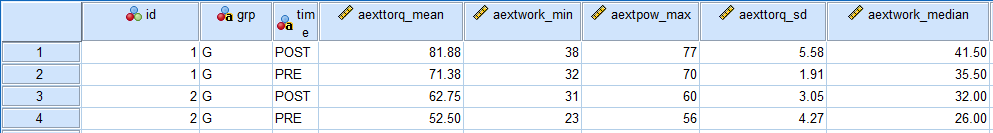
\includegraphics[width=1\linewidth]{images/aggregate} \caption{Aggregated summary}\label{fig:aggregate}
\end{figure}

\hypertarget{trick-8---group-by-function}{%
\chapter*{Trick 8 - Group by function}\label{trick-8---group-by-function}}
\addcontentsline{toc}{chapter}{Trick 8 - Group by function}

Many times you want to do the same thing repeatedly on certain chunks of data. For example, you want to find the mean strength on each level of sex (male, female), or even each level of the combination of sex-side (male-right, male-left, female-right, female-left). Precede whatever function you want to execute, with the command below. In the command below, I want to do the same analysis for each level of the combination of \texttt{grp} and \texttt{side}. This works for categorical variables. Replace \texttt{grp} and \texttt{side} with however many variables you want to split the data by.

\emph{PS} This means you can run the same stats on each split of the data by running the stats only once if you use this command.

Highlight this command and press the play button.

\begin{Shaded}
\begin{Highlighting}[]
\NormalTok{SORT CASES  BY grp side.}
\NormalTok{SPLIT FILE SEPARATE BY grp side.}
\end{Highlighting}
\end{Shaded}

After grouping the data, when I ran a descriptive analysis, this is what the results looks like in Figure \ref{fig:group-by}.

\begin{figure}
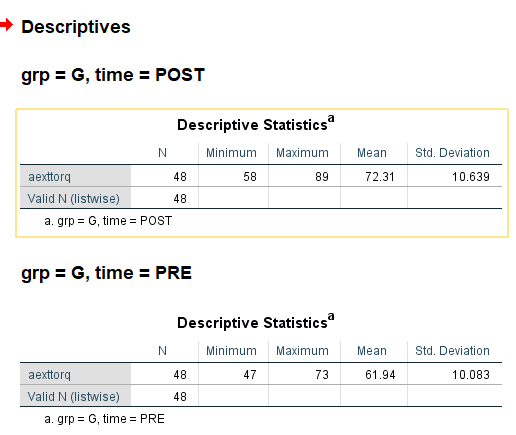
\includegraphics[width=0.6\linewidth]{images/group-by} \caption{Group-by descriptives}\label{fig:group-by}
\end{figure}

\hypertarget{trick-9---wide-to-long}{%
\chapter*{Trick 9 - Wide to long}\label{trick-9---wide-to-long}}
\addcontentsline{toc}{chapter}{Trick 9 - Wide to long}

\begin{figure}
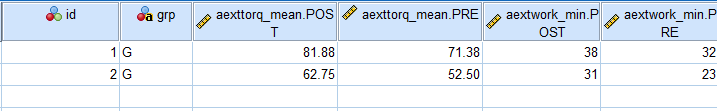
\includegraphics[width=1\linewidth]{images/wide_data} \caption{Wide data}\label{fig:ugly}
\end{figure}

Typically data is keyed into Excel in the wide format like in Figure \ref{fig:ugly}. In \textgreater{} 90\% of any data analysis, data should \textbf{NOT} be in this format. The only thing I know in SPSS that requires data to be in the wide format is when you want to use Repeated Measures Anova or a Paired t test. So it is useful to know how to convert a data to a long format since \textgreater{} 90\% of SPSS function requires data to be in a long format.

\texttt{/MAKE\ val\ FROM\ aexttorq\_pre\ aexttorq\_post} says collect all the variables \texttt{aexttorq\_pre}, \texttt{aexttorq\_post} and stack their values on top of each other. The column containing the values is called \texttt{val}. The column where the names of the values are stored is called \texttt{mediator}. Remember, you can call the new columns anything you want. \texttt{/KEEP=id\ grp\ time} simple says keep the following columns in the new data.

Highlight this command and press the play button.

\begin{Shaded}
\begin{Highlighting}[]
\NormalTok{VARSTOCASES}
  \SpecialCharTok{/}\NormalTok{MAKE val FROM aexttorq\_pre aexttorq\_post }
  \SpecialCharTok{/}\NormalTok{INDEX}\OtherTok{=}\FunctionTok{mediator}\NormalTok{(val) }
  \SpecialCharTok{/}\NormalTok{KEEP}\OtherTok{=}\NormalTok{id grp time}
  \SpecialCharTok{/}\ConstantTok{NULL}\OtherTok{=}\NormalTok{KEEP.}
\end{Highlighting}
\end{Shaded}

After running the command, this is what the results looks like in Figure \ref{fig:tidy}.

\begin{figure}
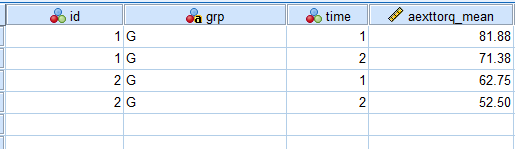
\includegraphics[width=1\linewidth]{images/long_data} \caption{Long data}\label{fig:tidy}
\end{figure}

\hypertarget{trick-10---long-to-wide}{%
\chapter*{Trick 10 - Long to wide}\label{trick-10---long-to-wide}}
\addcontentsline{toc}{chapter}{Trick 10 - Long to wide}

Just in case you need to make the data wide again. The two key commands are \texttt{/ID=id\ grp\ time} and \texttt{/INDEX=mediator}. \texttt{/ID} represents how each data point will be uniquely identified. \texttt{/INDEX} represents the variable you want to spread by.

Notice that trick 10 and 9 are mirror images. the \texttt{/ID} command in trick 10 should be identical to the \texttt{/KEEP} in trick 9. The \texttt{/INDEX} in both tricks 10 and 9 should contain the variable name you want to spread by.

\begin{Shaded}
\begin{Highlighting}[]
\NormalTok{CASESTOVARS}
  \SpecialCharTok{/}\NormalTok{ID}\OtherTok{=}\NormalTok{id grp time}
  \SpecialCharTok{/}\NormalTok{INDEX}\OtherTok{=}\NormalTok{mediator}
  \SpecialCharTok{/}\NormalTok{GROUPBY}\OtherTok{=}\NormalTok{VARIABLE.}
\end{Highlighting}
\end{Shaded}

After running the command, the data looks like in Figure \ref{fig:ugly} again.

  \bibliography{book.bib}

\end{document}
